\documentclass{article}
\usepackage[letterpaper, margin =1in]{geometry}
\usepackage[utf8]{inputenc}
\usepackage{amsmath}
\usepackage{graphicx}
\usepackage{array}
\usepackage{comment}
\usepackage{subfigure}

\title{CSC411 Project 1 - Face Recognition and Gender Classification with Regression}
\author{Che Liu, 1002246839}
\date{January 2018}

\begin{document}

\maketitle

\section*{A Note on Reproducing the Results}
A zip file containing all the required documents and scripts was submitted for this project. The zip file consists of one pdf report named faces.pdf, one tex file named faces.tex, five py scripts, and two folders named final\_male and final\_female. The five .py files are get\_data.py, part3.py, part5.py, part6.py, and part7.py. 
\par get\_data.py downloads the images necessary for this project and processes them so that they are usable for later parts. part3.py contains the code for Part 3 and Part 4 of this project. part5.py and part6.py contains the code for their respective parts. part7.py contains the code for Part 7 and Part 8 of this project. 
\par Since all the paths are relative, all the codes should be able to run in any directory. If you wish to use the zip file containing all the processed images instead of downloading them, please move the two folders (final\_male and final\_female) to the same directory where you intend to run the Python scripts. All other scripts should be able to run properly after that.

\section*{Part 1}
The images downloaded from the URLs provided in facescrub$\_$actors.txt and facescrub$\_$actresses.txt are of different sizes, angles, and color scales. Before cropping, converting to grayscale, and rescaling the images, the dataset of faces was composed of 1742 images of which 855 were of actors and 887 were of actresses. After manipulations mentioned above, the usable dataset shrink to 1688 images of which 834 were of actors and 854 were of actresses. The shrinkage was caused by factors such as invalid images. The exact sizes of the usable datasets for each actor and actress is shown in the table below:

\begin{center}
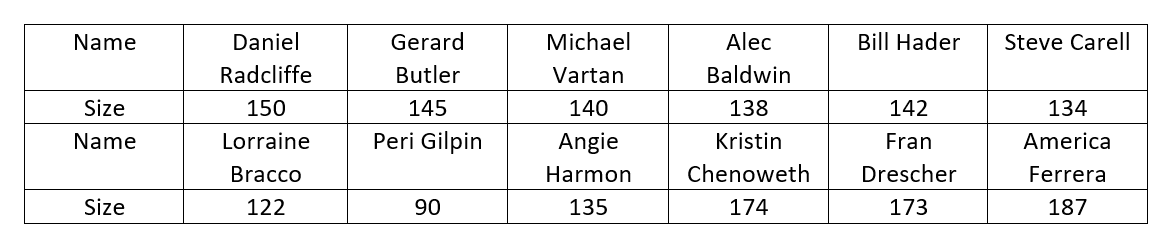
\includegraphics[width=1\textwidth]{DataSetSize.png}\\
Figure 1. Sizes of usable images of actors and actresses.
\end{center}

Three examples of the images in the original dataset are as follows:
\begin{center}
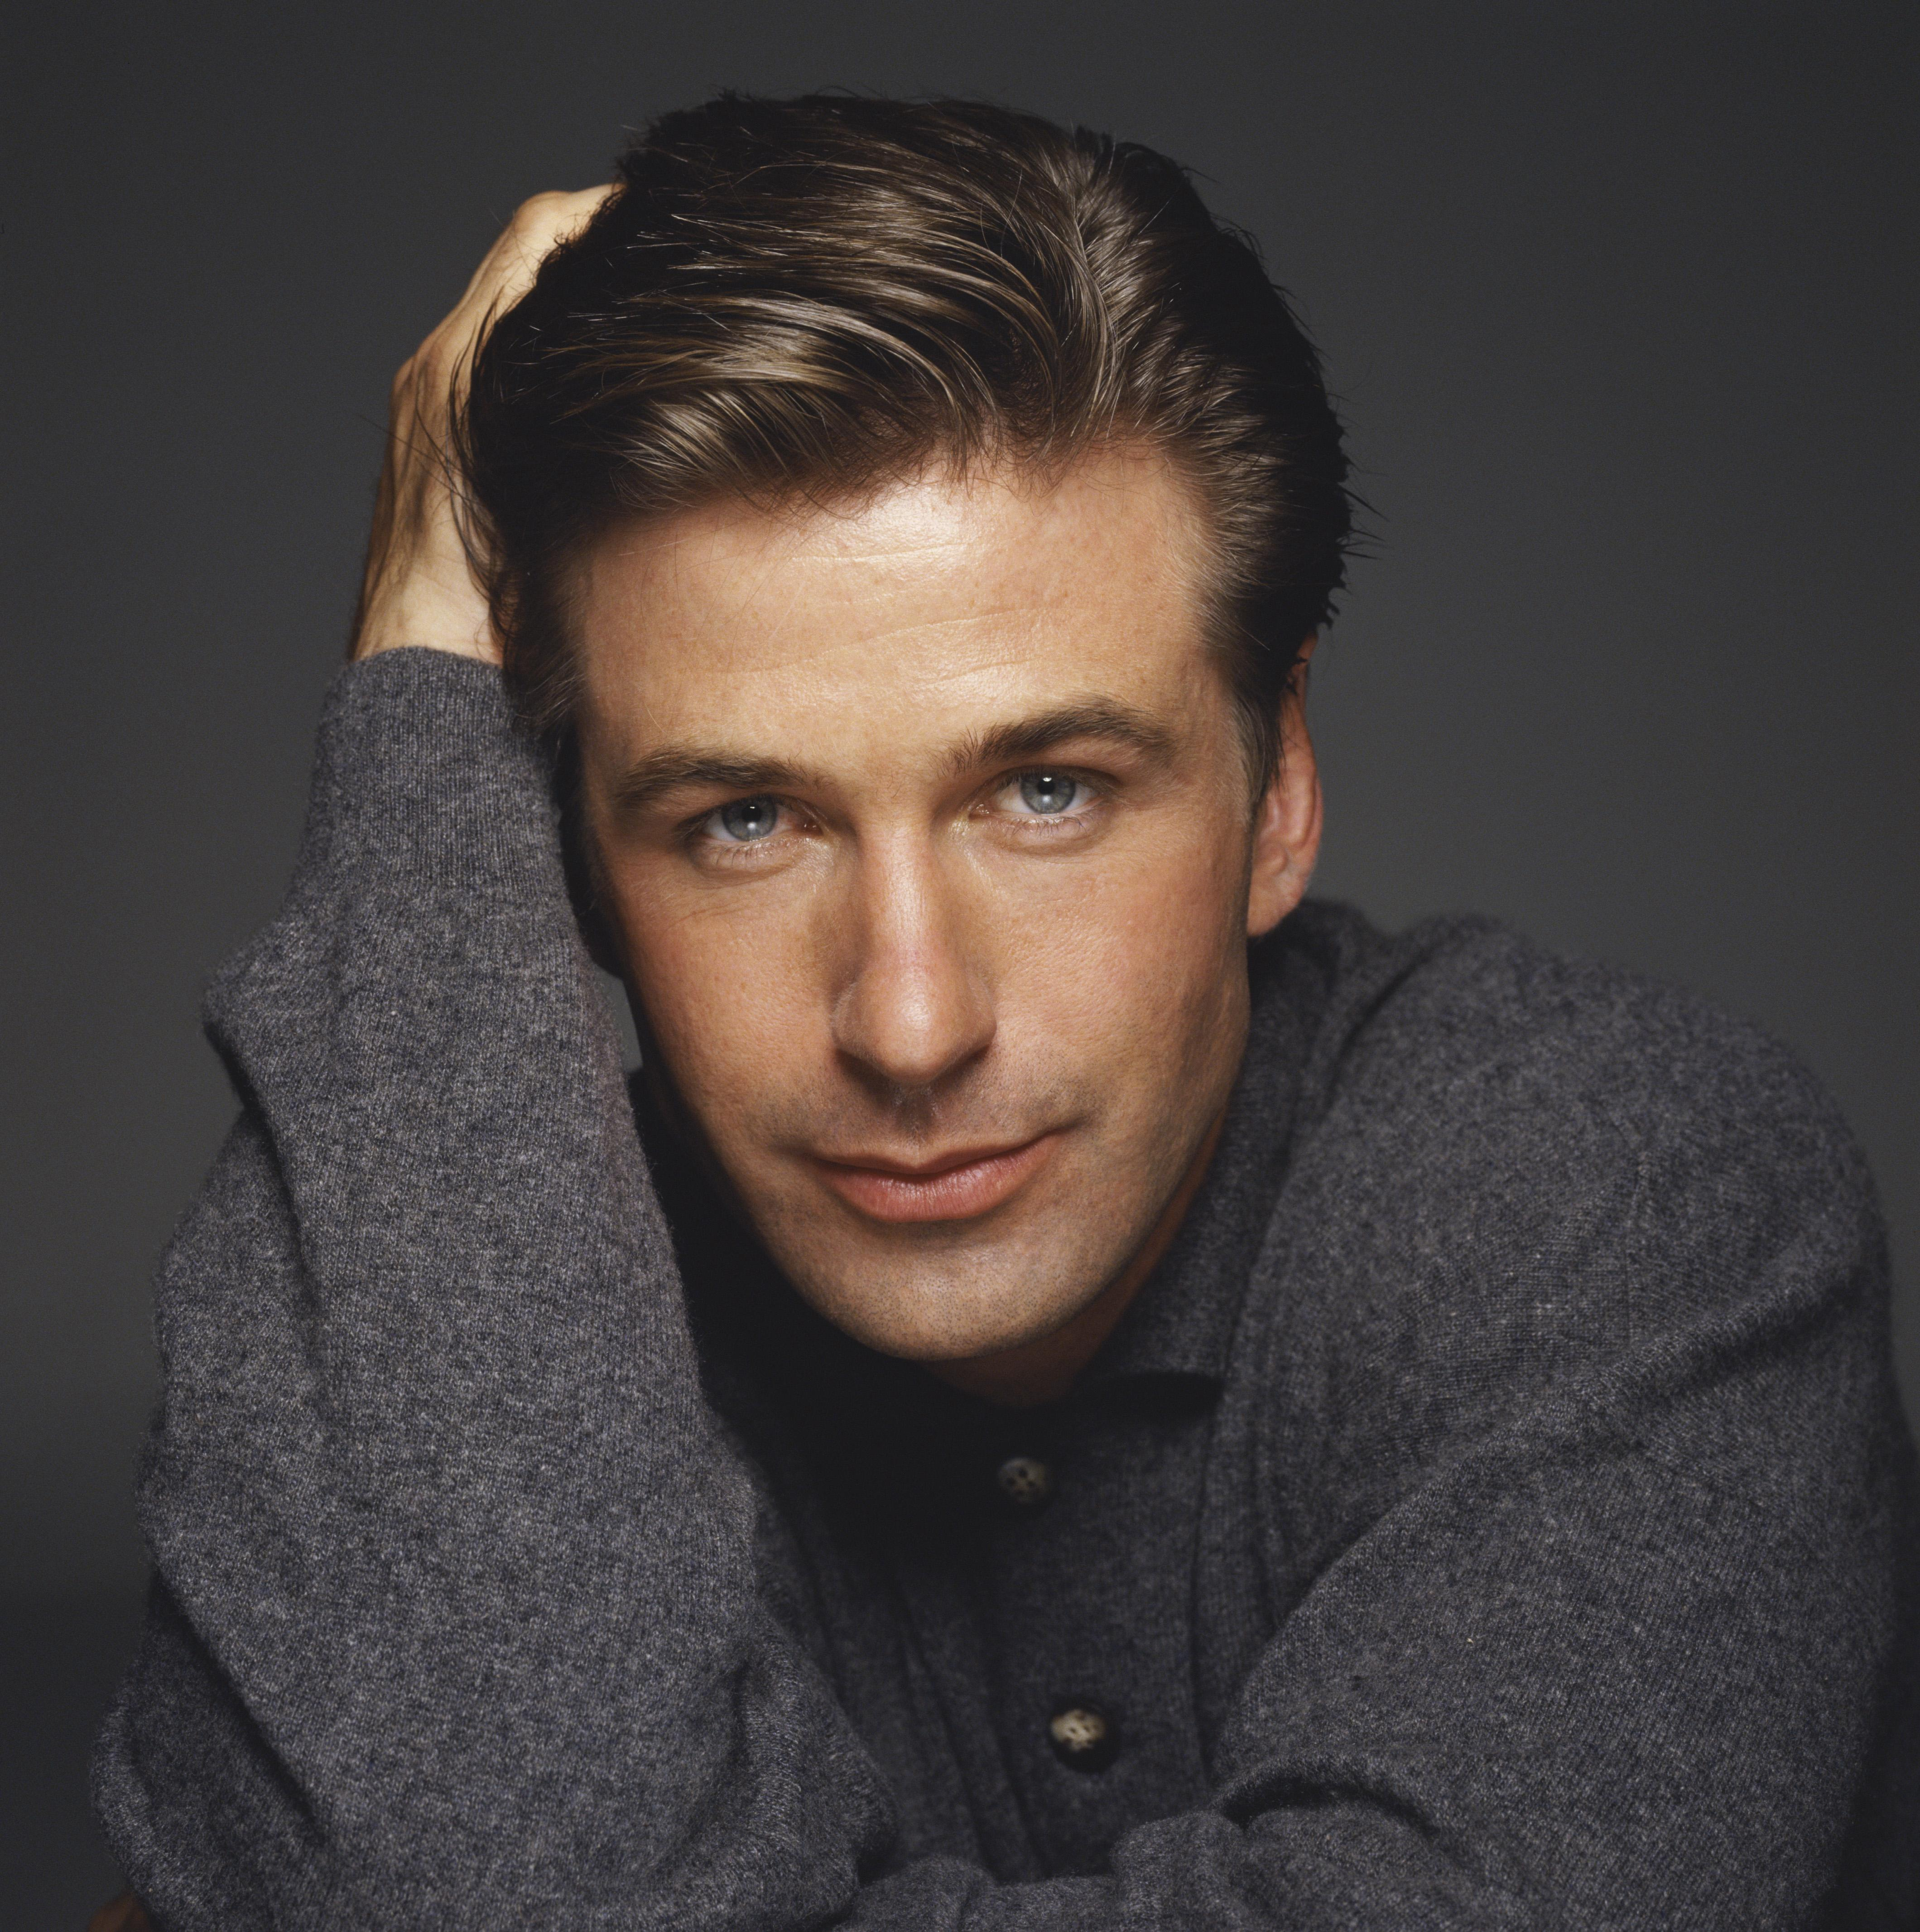
\includegraphics[width=0.4\textwidth]{OriginalBaldwin.jpg}\\
Figure 2. Original image of Alec Baldwin in the dataset.
\end{center}
\begin{center}
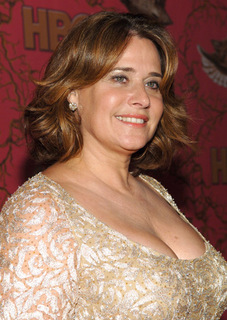
\includegraphics[width=0.4\textwidth]{OriginalBracco.jpg}\\
Figure 3. original image of Lorraine Bracco in the dataset.
\end{center}
\begin{center}
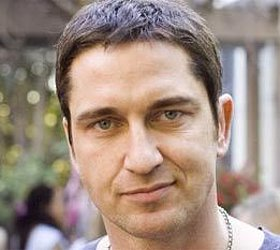
\includegraphics[width=0.4\textwidth]{OriginalButler.jpg}\\
Figure 4. Original image of Gerard Butler in the dataset.
\end{center}

Three examples of the cropped out faces are as follows:
\begin{center}

\includegraphics[width=0.3\textwidth]{CroppedBracco.jpg}\\
Figure 5. Cropped image of Lorraine Bracco in the dataset.
\end{center}
\begin{center}

\includegraphics[width=0.3\textwidth]{CroppedChenoweth.jpg}\\
Figure 6. Cropped image of GKristin Chenoweth in the dataset.
\end{center}
\begin{center}

\includegraphics[width=0.3\textwidth]{CroppedCarell.jpg}\\
Figure 7. Cropped image of Steve Carell in the dataset.
\end{center}

The bounding boxes are accurate for the vast majority of images. Quantitatively, the faces in only 7 out of 1688 cropped images are incomplete or absent. Two of such examples are baldwin67.jpg and carell93.jpeg. The former is shown below:
\begin{center}
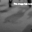
\includegraphics[width=0.3\textwidth]{baldwin67.jpg}\\
Figure 8. Baldwin67.jpg with incorrect bounding box.
\end{center}

\par The cropped out faces are mostly aligned with each other. In some images, however, the actor/actress is not facing the camera or is tilting his/her head. In some images, the actor/actress wears glasses, which may have a slight impact on the accuracy of regression. An example in which the actor is not facing forward is shown below:
\begin{center}

\includegraphics[width=0.3\textwidth]{carell89.jpg}\\
Figure 9. Carell89.jpg in which the actor's face does not align with others.
\end{center}

\section*{Part 2}
90 images need to be selected for each actor/actress without overlapping. More specifically, 70 images for training, 10 for validation, and 10 for testing need to be chosen by means of randomness. The algorithm used is as follows:

\begin{itemize}
    \item Initialize twelve empty lists corresponding to the twelve actors/actresses.
    \item Append the file names of all the cropped images to their corresponding lists.
    \item (Call np.random.seed (0) such that the result is reproducible.)
    \item To avoid potential bias, shuffle the lists using np.random.shuffle () for randomization.
    \item Initialize three more lists for each actor/actress, corresponding to the training, validation, and testing sets.
    \item For each list corresponding to the training set, pop the list containing all file names of images of that actor/actress 70 times and append to the training list.
    \item For each list corresponding to the validation set, pop the list containing all file names of images of that actor/actress 10 times and append to the validation list.
    \item For each list corresponding to the test set, pop the list containing all file names of images of that actor/actress 10 times and append to the test list.
\end{itemize}

\section*{Part 3}
Linear regression is used to classify the images as of Alec Baldwin or Steve Carell, the following quadratic loss function is minimized:
\begin{equation}
   J(\theta) = \sum_i{(y^{(i)}-\theta^{T}x^{(i)})^2}
\end{equation}
where $x^{(i)}$ corresponds to the pixel intensities of the $i^{th}$ image divided by 255.0 of a particular image ($x_0 = 1$ for the offset $\theta_0$), $y^{(i)}$ is the label of the image, $\theta^T$ = [$\theta_0$ $\theta_1$ ... $\theta_{1024}$] is the coefficients we need to run gradient descent on. $h_{\theta} = \theta^Tx$ is the hypothesis.

\par The values of this cost function on training and validation sets are f(x) = 0.58813 and f(x) = 6.49813, respectively. This is consistent with our intuition since the tuned model fits the training set better than the validation set.
\par Performance-wise, the classifier can correctly classify 100\% of images in the training set and 95\% of images in the validation set.
\par Images of Baldwin and Carell are mapped to values of +1's and -1's, respectively. Thus, if the result of $\theta^{T}x^{(i)}$ is greater than 0, the algorithm believes that it is more probable for the image to be of Baldwin. And if the result is smaller than 0, the algorithm believes that it is more probable that the image is of Carell.
\par The code of the function used to compute the output of the classifier (on validation set) is as follows:
\begin{center}
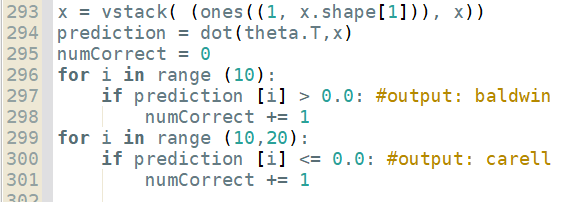
\includegraphics[width=0.7\textwidth]{ValidationOutput.png}\\
Figure 10. the function used to classify the output as Baldwin or Carell.
\end{center}
\par There are several factors that affect the performance of this classifier. In particular, a learning rate ($\alpha$) that is too high can result in overflow which crashes the gradient descent algorithm, an indication that gradient descent does not converge. On the other hand, if the learning rate is set too low, gradient descent may converge too slowly or simply not be able to run many steps due to the EPS, although the cost function is convex and getting trapped in a local minimums is not a problem. What I did was starting from a rather large learning rate, and reduce the learning rate to half if the gradient descent algorithm crashes or the loss function ended up too big. I kept doing this until the loss cannot be reduced noticeably and the performance on both the training set and validation set are high. By then, the image generated by the $\theta$'s looks somewhat, but not overly resembles a face.
\par If I decrease EPS and increase the maximum number of iterations, gradient descent will produce $\theta$'s which models the training set more closely. However, this may result in a decrease in the performance on the validation set due to over-fitting. The approach I adopted was similar as before. I gradually increased the maximum number of interactions and decreased EPS such that the performance on the validation set did not decrease due to overfitting.
\par Furthermore, theta0 is drawn from a normal distribution centered at zero. Since the quadratic loss function is convex, its only minimum is its global minimum. The selection of theta0 need to minimize the initial cost of the cost function. By trying out normal distributions with different standard deviations centered at zero, it was found that the initial loss is generally minimized when the standard deviation is 0, or, in other words, when theta0 is all zeros.


\newpage
\section*{Part 4}
In this part, the coefficients $\theta_{1}$ to $\theta_{1025}$ gotten from gradient descent are reshaped into a 32x32 matrix. This matrix is read as pixel intensities and displayed using the plt.imread () and plt.imshow () functions.
\subsection*{(a)}
Using full training dataset (70 images per actor), the following image is obtained:
\begin{center}
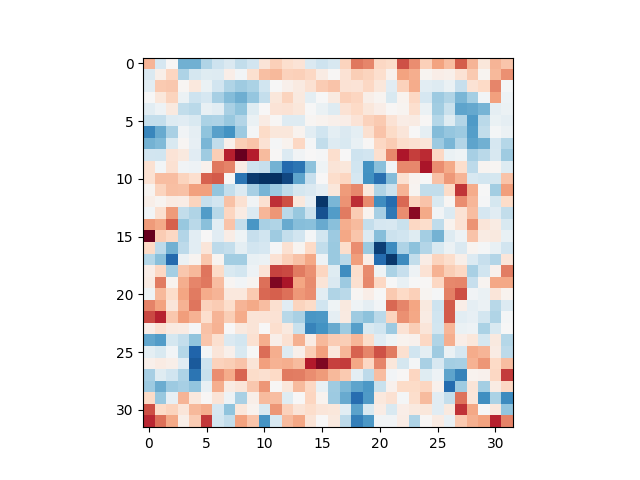
\includegraphics[width=0.6\textwidth]{Theta70.png}\\
Figure 11. Visualization of the $\theta$'s obtained using full training set.
\end{center}


Using two images for each actor, the following image is obtained:

\begin{center}
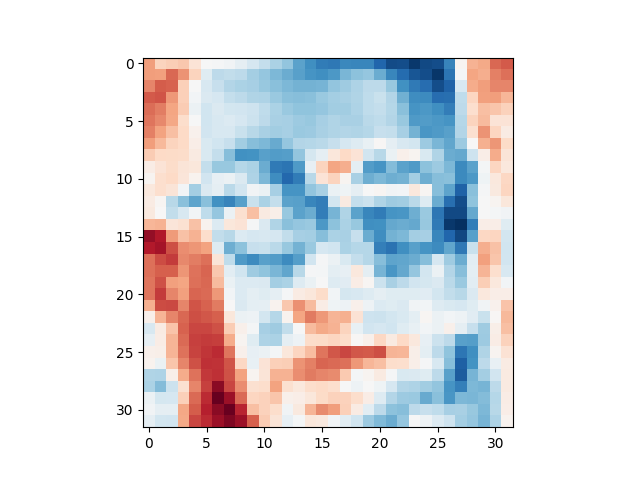
\includegraphics[width=0.6\textwidth]{Theta2.png}\\
Figure 12. Visualization of the $\theta$'s obtained using two images of each actor.
\end{center}

\newpage
\subsection*{(b)}
In this part, we will obtain both a visualization that contains a face and a visualization that does not, using full training set (70 images for each actor). 
It was noticed that as stopping gradient descent earlier and earlier by setting the maximum number of iterations to a smaller and smaller value, the image resulting from the $\theta$'s looked increasingly like a face. 
\par If I set the maximum number of iteration to 1000, the following visualization is obtained using the full training set:
\begin{center}
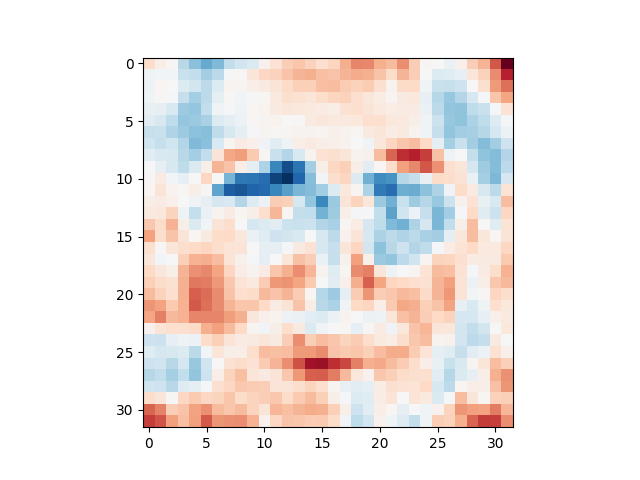
\includegraphics[width=0.6\textwidth]{part4b1000.png}\\
Figure 13. Visualization of the $\theta$'s obtained by ending gradient descent early. 
\end{center}
\par On the other hand, if we end gradient descent later by setting the maximum number of iterations to a greater value and the EPS to a smaller value, visualization looked less like a face.
\par When I set the EPS to 1e-10 and the maximum number of iterations to 200000, the following visualization is obtained:
\begin{center}
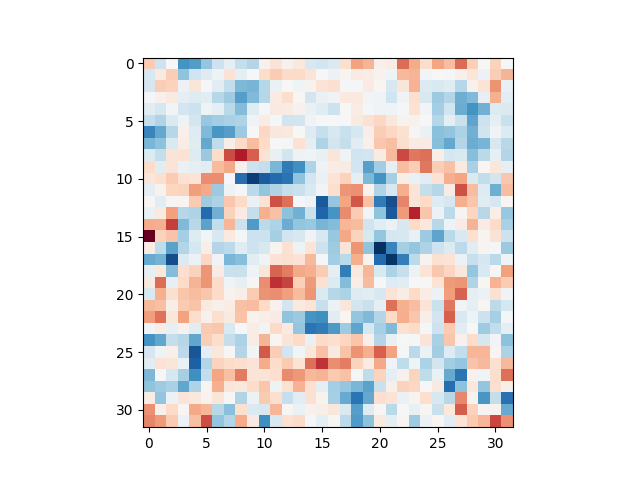
\includegraphics[width=0.6\textwidth]{part4b200000.png}\\
Figure 14. Visualization of the $\theta$'s obtained by ending gradient descent late. 
\end{center}

\par Furthermore, theta0 also has an effect on whether the visualization appears to be a face. It seems that if we increase the standard deviation/variance of the normal distribution from which we draw theta0, the visualization looks more random. In particular, if we set the standard deviation to 0.1, while keeping the mean 0 (and restore all other settings back to those used in part 3), we get the following visualization: 
\begin{center}
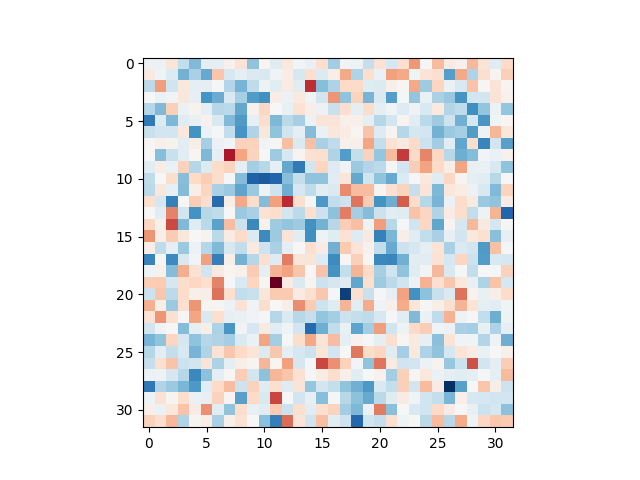
\includegraphics[width=0.6\textwidth]{part4bSD01.png}\\
Figure 15. Visualization of the $\theta$'s obtained by increasing standard deviation. 
\end{center}
In contrast, if we keep the distribution as N(0.,0.), the following visualization is obtained:
\begin{center}
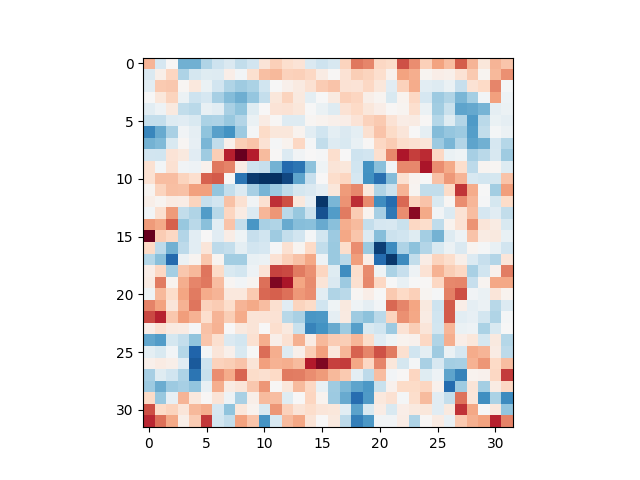
\includegraphics[width=0.6\textwidth]{part4bNormal.png}\\
Figure 16. Visualization of the $\theta$'s obtained by having 0 standard deviation. 
\end{center}



\newpage
\section*{Part 5}
Images are classified as of male or female in this part. To demonstrate overfitting, the percentages of images correctly classified on the training, validation, and unknown sets when the size of training set is between 40 and 200 (per gender) are plotted in increments of 10. The plot is shown below:
\begin{center}
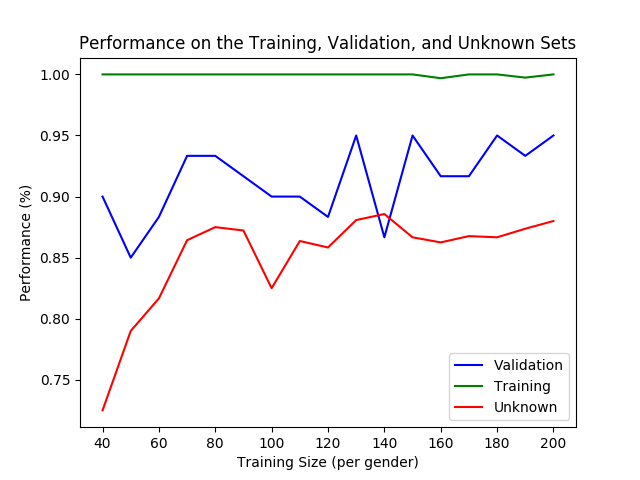
\includegraphics[width=0.7\textwidth]{part5result.png}\\
Figure 17. Performances of the gender classifier on the training, validation, and unknown set against size of the training set.
\end{center}
As can be clearly see, the percentage of images correctly classified on the validation and unknown sets steadily increases as the number of images we used to train the classifier increases. Specifically, the performances increased from around 85\% and 70\% for the validation and unknown sets to around 95\% and 85\%, respectively in this particular run. Nevertheless, the performance of the classifier on the training set drops slightly as we increase the size of training set.
\par The performance of the classifier on the validation and unknown sets are determined by the number of images correctly classified out of only sixty images hence explains the fluctuation. However, the raising trends on the validation and unknown sets are obvious to see.
\par Overfitting is an issue when the size of the training set is small, since the classifier models a small portion of the  full training set more closely hence fails to model other images. The predictive power of the classifier is low when the size of the training set is small, because the performance on the training set ($\approx100\%$) is significantly better than that on the validation/unknown sets ($\approx80\%$).  As the size of the training set increases, the performance also steadily increases because overfitting is less and less of a problem.
\par By the same reason, the performance of the classifier also increases on the actors not included in \textit{act} when the size of the training set increases. In particular, when 200 images are used to train the classifier, around 95\% of validation sets are correctly classified based on gender. 
\par The maximum number of iterations is manually decreased to 10000 from 30000 to reduce the time it takes to run the program. 

\newpage
\section*{Part 6}
\subsection*{a)}
\begin{center}
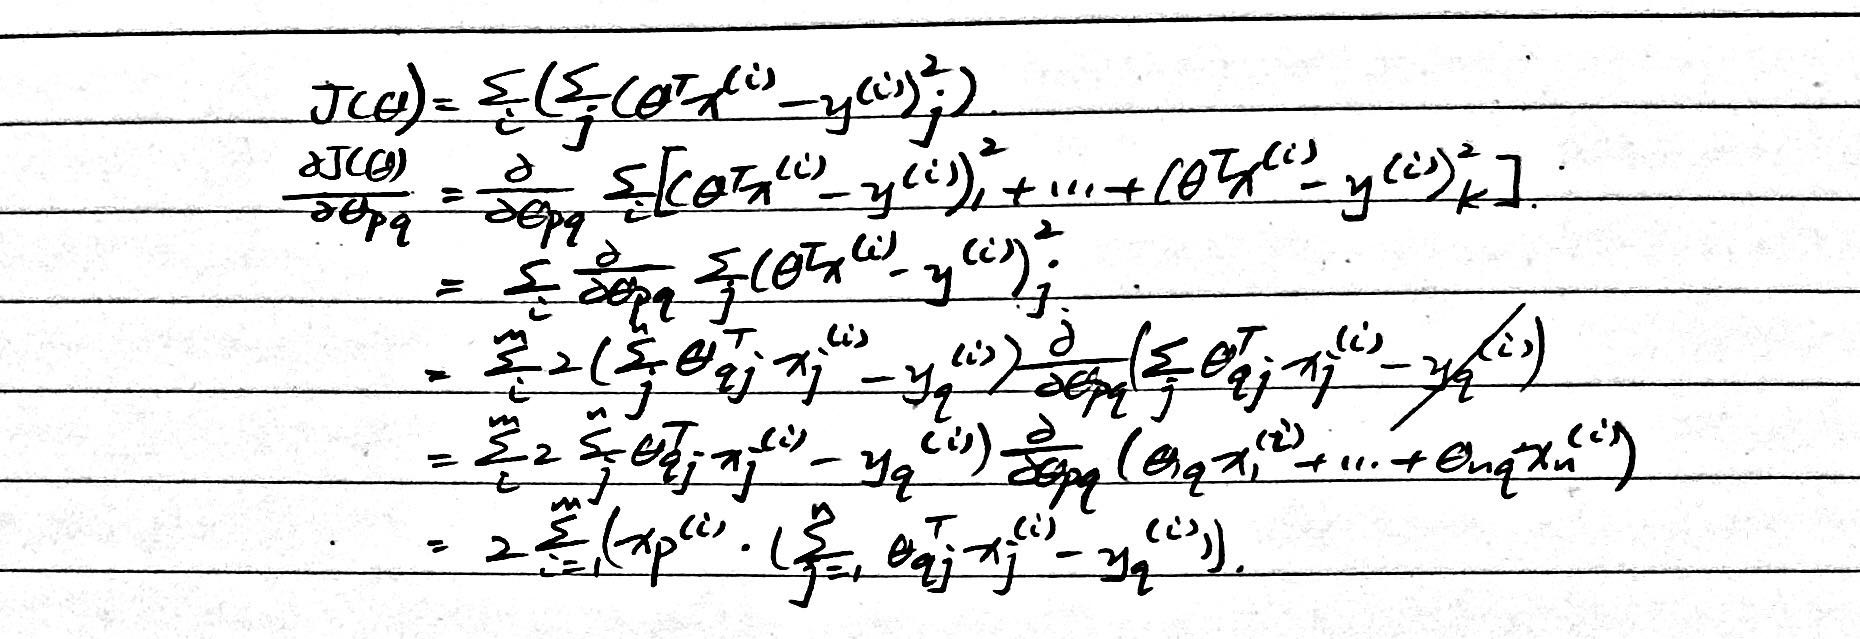
\includegraphics[width=1\textwidth]{part6a.jpeg}\\
\end{center}

As can be seen from the deviation above: 
\begin{equation}
    \frac{\partial J}{\partial \theta_{pq}} = 2\sum_{i=1}^{m}(x_p^{(i)}\sum_{j=1}^{n}(\theta_{qj}^Tx_j^{(i)}-y_q^{(i)}))
\end{equation}

\subsection*{b)}
\begin{center}
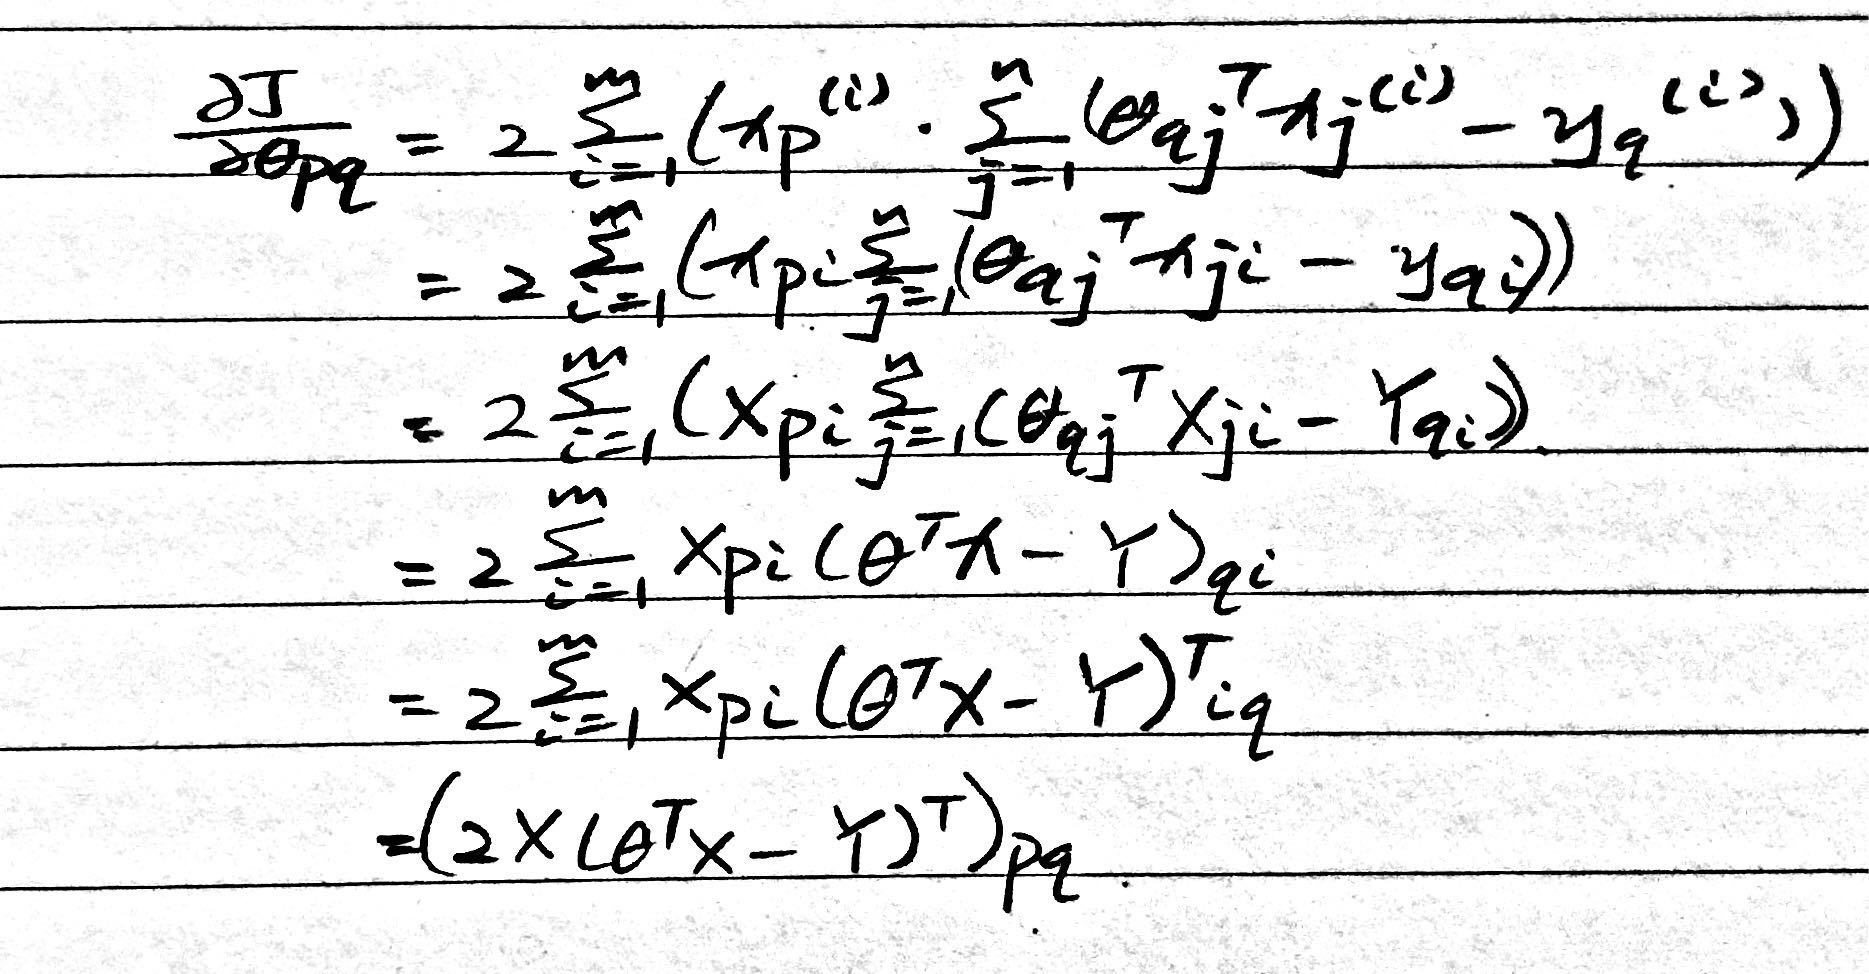
\includegraphics[width=0.7\textwidth]{part6b.jpeg}\\
\end{center}

\begin{center}
Dimensions:\\
X: $n\times m$\\
Y: $k\times m$\\
$\theta$: $n\times k$\\
where m is the number of training examples, n is the number of features (pixels) in each image (1025 including the bias term), k is the number of outputs.
\end{center}
\newpage
\subsection*{c)}
The implementation of the cost function from Part 6(a) and its vectorized gradient function in Python is shown below:
\begin{center}
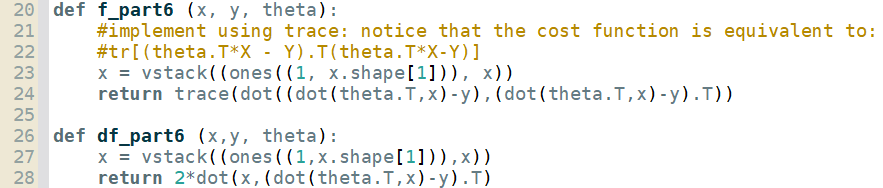
\includegraphics[width=1\textwidth]{part6c.png}\\
Figure 18. Python code for implementing the f and df functions. 
\end{center}

\subsection*{(d)}
Finite difference approximation is used to demonstrate that the implementation of the gradient function is correct. The following code is used to calculate the finite difference approximation:\\
\begin{left}
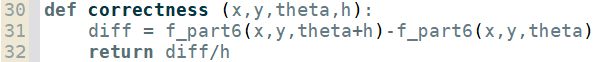
\includegraphics[width=0.6\textwidth]{finiteDiff.png}
\end{left}
\begin{center}
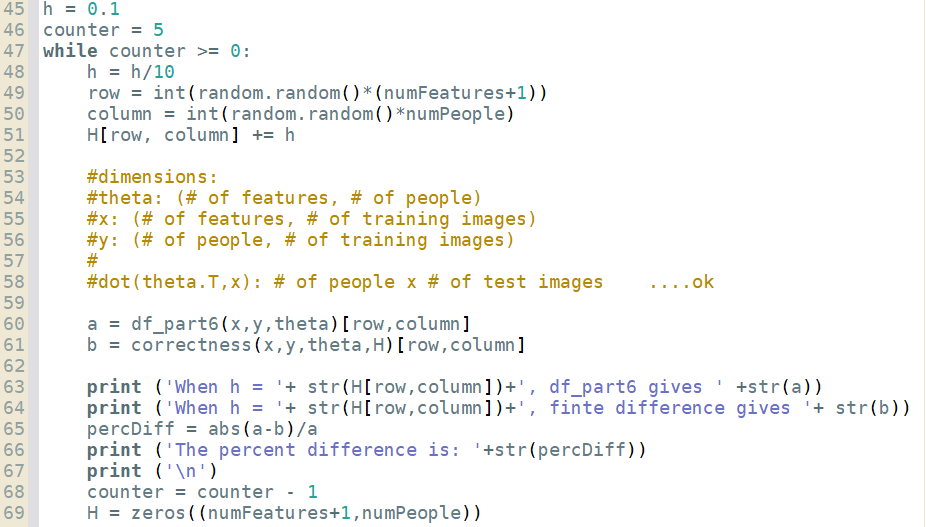
\includegraphics[width=1\textwidth]{part6d.png}\\
Figure 19. Python code for verifying the correctness of df. 
\end{center}

In terms of selecting h, any h that is not too big and does not cause a numerical issue is acceptable.The output of this part is plotted for better visualization of the trend: 
\begin{center}
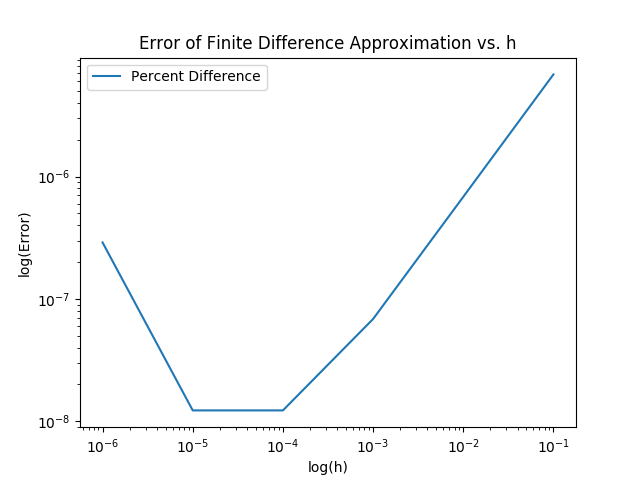
\includegraphics[width=0.7\textwidth]{part6d2.png}\\
Figure 20. Graph of log (Error) and log (h) for visualizing the trend.
\end{center}

\section*{Part 7}
In this part, the classifier is trained to distinguish the six actors/actresses in the list act.\\
\par The performance that the classifier obtained on the training set is 97.38\%\\
\par The performance that the classifier obtained on the validation set is 81.67\%\\
\par A learning rate of 0.000001, EPS of 10e-5, max-iteration of 30000, and theta0 of all zeros are chosen using the same method as described in part 3. The value seems to make sense considering the performance on the validation set is excellent. If the algorithm simply guesses which actor/actress is in the picture, it would have a chance of merely 16.67\% to get the correct answer. Given that the classifier gets 76.67\% of the images correct in the validation set, clearly the algorithm is working hence gradient descent must be functioning as well.
\par Since one-hot coding is used to label the images when we generated y, to obtain the label in the classifier's prediction, we simply read $\theta^Tx$ column by column, each of which corresponds to an image we want to find the predicted label of. The maximum value in each column indicates which actor/actress the classifier predicts. For instance, suppose a column in the output of the hypothesis function is [0.1, 0.5, 0.7, 0.4, 0.2, 0.9], it is an indication that the classifier classifies the image as one of Carell. This is because 0.9 is the highest value in the row, meaning the corresponding actor/actress is the most probable. The code used to achieve this functionality is given below: (I took the transpose of the hypothesis/prediction matrix so that it is easier to work with)
\begin{center}
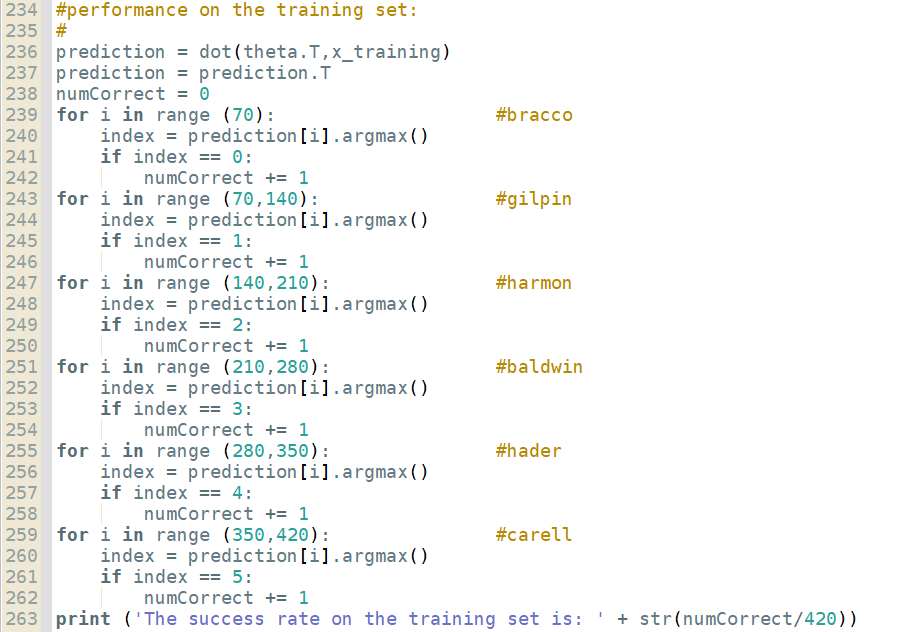
\includegraphics[width=0.9\textwidth]{part7Code.png}\\
Figure 21. Python code used for testing if the predictions are correct.
\end{center}

\newpage
\section*{Part 8}
We can get the $\theta$ visualization for each actor/actress by converting the corresponding column of $\theta$ to a 32x32 matrix and using the imread() function. The results are as shown in the images below:
\begin{center}
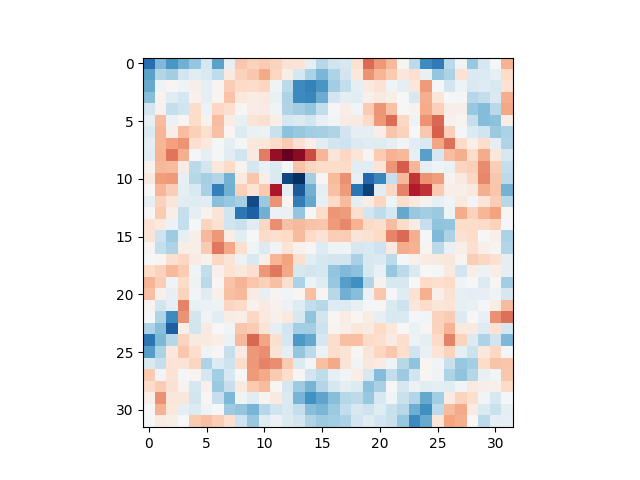
\includegraphics[width=0.6\textwidth]{part8Bracco.png}\\
Figure 22. $\theta$ visualization for Bracco.
\end{center}

\begin{center}
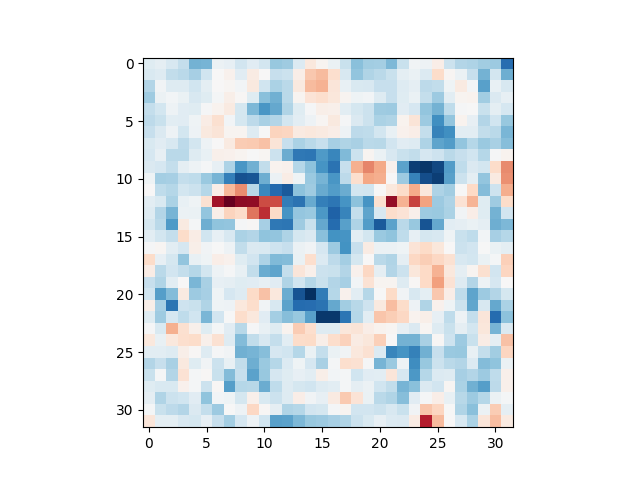
\includegraphics[width=0.6\textwidth]{part8Gilpin.png}\\
Figure 23. $\theta$ visualization for Gilpin..
\end{center}

\begin{center}
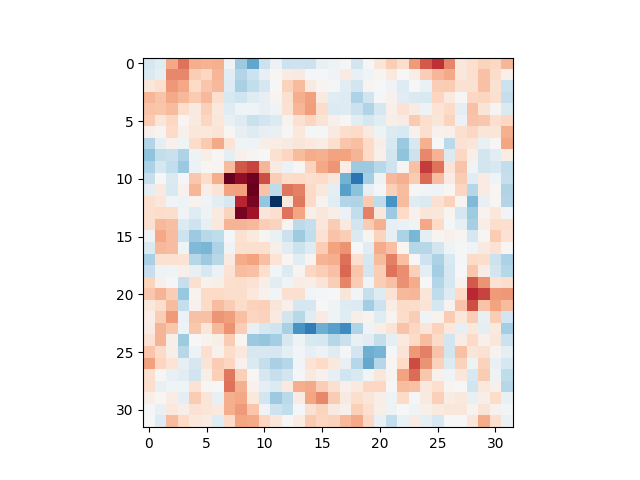
\includegraphics[width=0.6\textwidth]{part8Harmon.png}\\
Figure 24. $\theta$ visualization for Harmon.
\end{center}

\begin{center}
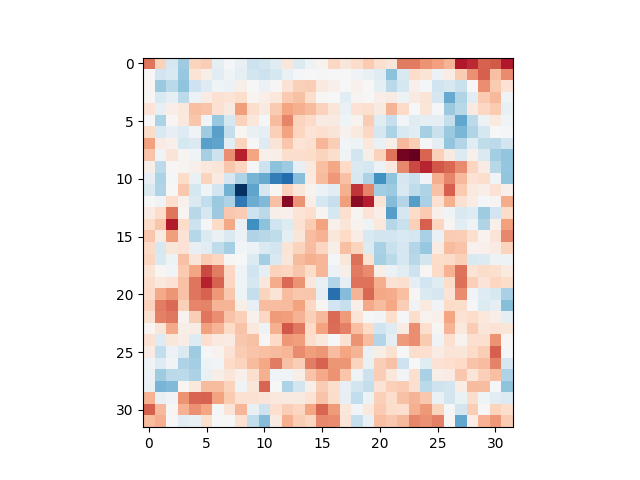
\includegraphics[width=0.6\textwidth]{part8Baldwin.png}\\
Figure 25. $\theta$ visualization for Baldwin.
\end{center}

\begin{center}
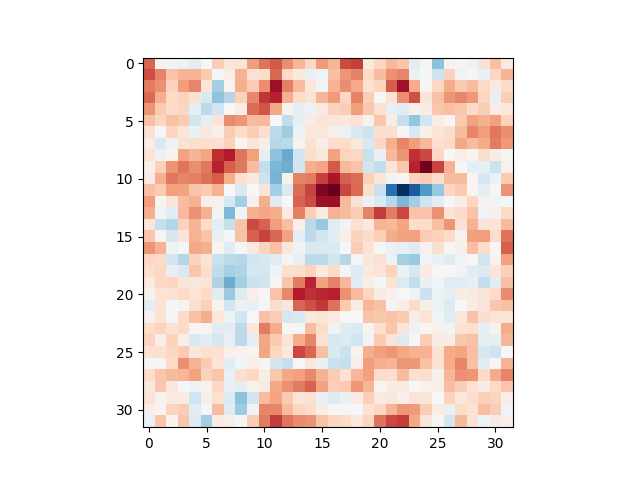
\includegraphics[width=0.6\textwidth]{part8Hader.png}\\
Figure 26. $\theta$ visualization for Hader.
\end{center}

\begin{center}
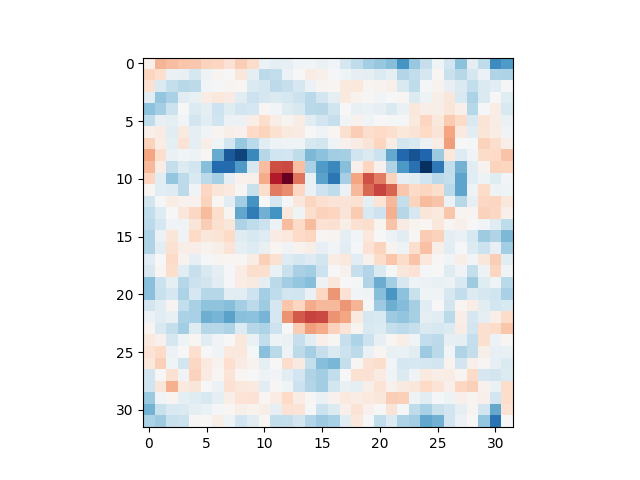
\includegraphics[width=0.6\textwidth]{part8Carell.png}\\
Figure 27. $\theta$ visualization for Carell.
\end{center}

\end{document}
